\chapter{Kombinatoriikka}

\index{kombinatoriikka@kombinatoriikka}

\key{Kombinatoriikka} tarkoittaa yhdistelmien määrän laskemista.
Yleensä tavoitteena on toteuttaa laskenta
tehokkaasti niin, että jokaista yhdistelmää
ei tarvitse muodostaa erikseen.

Tarkastellaan esimerkkinä tehtävää,
jossa laskettavana on,
monellako tavalla luvun $n$ voi esittää positiivisten
kokonaislukujen summana.
Esimerkiksi luvun 4 voi esittää 8 tavalla
seuraavasti:
\begin{multicols}{2}
\begin{itemize}
\item $1+1+1+1$
\item $1+1+2$
\item $1+2+1$
\item $2+1+1$
\item $2+2$
\item $3+1$
\item $1+3$
\item $4$
\end{itemize}
\end{multicols}

Kombinatorisen tehtävän ratkaisun voi usein
laskea rekursiivisen funktion avulla.
Tässä tapauksessa voimme määritellä funktion $f(n)$,
joka laskee luvun $n$ esitystapojen määrän.
Esimerkiksi $f(4)=8$ yllä olevan esimerkin mukaisesti.
Funktion voi laskea rekursiivisesti seuraavasti:
\begin{equation*}
    f(n) = \begin{cases}
               1               & n = 1\\
               f(1)+f(2)+\ldots+f(n-1)+1 & n > 1\\
           \end{cases}
\end{equation*}
Pohjatapauksena on $f(1)=1$,
koska luvun 1 voi esittää vain yhdellä tavalla.
Rekursiivinen tapaus käy läpi
kaikki vaihtoehdot,
mikä on summan viimeinen luku.
Esimerkiksi tapauksessa $n=4$ summa voi päättyä
$+1$, $+2$ tai $+3$.
Tämän lisäksi lasketaan mukaan esitystapa,
jossa on pelkkä luku $n$.

Funktion ensimmäiset arvot ovat:
\[
\begin{array}{lcl}
f(1) & = & 1 \\
f(2) & = & 2 \\
f(3) & = & 4 \\
f(4) & = & 8 \\
f(5) & = & 16 \\
\end{array}
\]
Osoittautuu, että funktiolle on myös suljettu muoto
\[
f(n)=2^{n-1},
\]
mikä johtuu siitä, että summassa on $n-1$ mahdollista
kohtaa +-merkille ja niistä valitaan mikä tahansa osajoukko.

\section{Binomikerroin}

\index{binomikerroin@binomikerroin}

\key{Binomikerroin} ${n \choose k}$ ilmaisee,
monellako tavalla $n$ alkion joukosta
voidaan muodostaa $k$ alkion osajoukko.
Esimerkiksi ${5 \choose 3}=10$,
koska joukosta $\{1,2,3,4,5\}$
voidaan valita $10$ tavalla $3$ alkiota:
\[ \{1,2,3\}, \{1,2,4\}, \{1,2,5\}, \{1,3,4\}, \{1,3,5\}, 
\{1,4,5\}, \{2,3,4\}, \{2,3,5\}, \{2,4,5\}, \{3,4,5\} \]

\subsubsection{Laskutapa 1}

Binomikertoimen voi laskea rekursiivisesti seuraavasti:

\[
{n \choose k}  =  {n-1 \choose k-1} + {n-1 \choose k}
\]

Ideana rekursiossa on tarkastella tiettyä
joukon alkiota $x$.
Jos alkio $x$ valitaan osajoukkoon,
täytyy vielä valita $n-1$ alkiosta $k-1$ alkiota.
Jos taas alkiota $x$ ei valita osajoukkoon,
täytyy vielä valita $n-1$ alkiosta $k$ alkiota.

Rekursion pohjatapaukset ovat seuraavat:

\[
{n \choose 0}  =  {n \choose n} = 1
\]

Tämä johtuu siitä, että on aina yksi tapa
muodostaa tyhjä osajoukko,
samoin kuin valita kaikki alkiot osajoukkoon.

\subsubsection{Laskutapa 2}

Toinen tapa laskea binomikerroin on seuraava:
\[
{n \choose k}  =  \frac{n!}{k!(n-k)!}.
\]

Kaavassa $n!$ on $n$ alkion permutaatioiden määrä.
Ideana on käydä läpi kaikki permutaatiot
ja valita kussakin tapauksessa
permutaation $k$ ensimmäistä alkiota osajoukkoon.
Koska ei ole merkitystä,
missä järjestyksessä osajoukon alkiot
ja ulkopuoliset alkiot ovat,
tulos jaetaan luvuilla $k!$ ja $(n-k)!$.

\subsubsection{Ominaisuuksia}

Binomikertoimelle pätee
\[
{n \choose k}  =  {n \choose n-k},
\]
koska $k$ alkion valinta osajoukkoon
tarkoittaa samaa kuin että valitaan
$n-k$ alkiota osajoukon ulkopuolelle.

Binomikerrointen summa on
\[
{n \choose 0}+{n \choose 1}+{n \choose 2}+\ldots+{n \choose n}=2^n.
\]

Nimi ''binomikerroin'' tulee siitä, että

\[ (a+b)^n =
{n \choose 0} a^n b^0 + 
{n \choose 1} a^{n-1} b^1 +
\ldots + 
{n \choose n-1} a^1 b^{n-1} +
{n \choose n} a^0 b^n. \]

\index{Pascalin kolmio}

Binomikertoimet esiintyvät myös \key{Pascalin
kolmiossa}, jonka reunoilla on lukua 1
ja jokainen luku saadaan
kahden yllä olevan luvun summana:
\begin{center}
\begin{tikzpicture}{0.9}
\node at (0,0) {1};
\node at (-0.5,-0.5) {1};
\node at (0.5,-0.5) {1};
\node at (-1,-1) {1};
\node at (0,-1) {2};
\node at (1,-1) {1};
\node at (-1.5,-1.5) {1};
\node at (-0.5,-1.5) {3};
\node at (0.5,-1.5) {3};
\node at (1.5,-1.5) {1};
\node at (-2,-2) {1};
\node at (-1,-2) {4};
\node at (0,-2) {6};
\node at (1,-2) {4};
\node at (2,-2) {1};
\node at (-2,-2.5) {$\ldots$};
\node at (-1,-2.5) {$\ldots$};
\node at (0,-2.5) {$\ldots$};
\node at (1,-2.5) {$\ldots$};
\node at (2,-2.5) {$\ldots$};
\end{tikzpicture}
\end{center}

\subsubsection{Laatikot ja pallot}

''Laatikot ja pallot'' on usein hyödyllinen malli,
jossa $n$ laatikkoon sijoitetaan $k$ palloa.
Tarkastellaan seuraavaksi kolmea tapausta:

\textit{Tapaus 1}: Kuhunkin laatikkoon saa sijoittaa
enintään yhden pallon.
Esimerkiksi kun $n=5$ ja $k=2$,
sijoitustapoja on 10:

\begin{center}
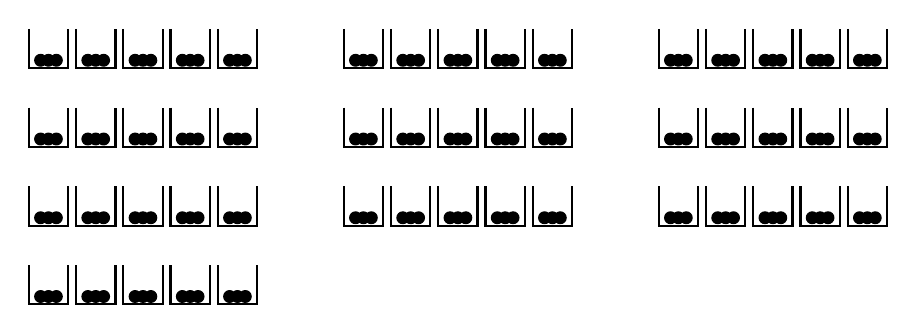
\begin{tikzpicture}[scale=0.5]
\newcommand\lax[3]{
\path[draw,thick,-] (#1-0.5,#2+0.5) -- (#1-0.5,#2-0.5) --
                    (#1+0.5,#2-0.5) -- (#1+0.5,#2+0.5);
\ifthenelse{\equal{#3}{1}}{\draw[fill=black] (#1,#2-0.3) circle (0.15);}{}
\ifthenelse{\equal{#3}{2}}{\draw[fill=black] (#1-0.2,#2-0.3) circle (0.15);}{}
\ifthenelse{\equal{#3}{2}}{\draw[fill=black] (#1+0.2,#2-0.3) circle (0.15);}{}
}
\newcommand\laa[7]{
    \lax{#1}{#2}{#3}
    \lax{#1+1.2}{#2}{#4}
    \lax{#1+2.4}{#2}{#5}
    \lax{#1+3.6}{#2}{#6}
    \lax{#1+4.8}{#2}{#7}
}

\laa{0}{0}{1}{1}{0}{0}{0}
\laa{0}{-2}{1}{0}{1}{0}{0}
\laa{0}{-4}{1}{0}{0}{1}{0}
\laa{0}{-6}{1}{0}{0}{0}{1}
\laa{8}{0}{0}{1}{1}{0}{0}
\laa{8}{-2}{0}{1}{0}{1}{0}
\laa{8}{-4}{0}{1}{0}{0}{1}
\laa{16}{0}{0}{0}{1}{1}{0}
\laa{16}{-2}{0}{0}{1}{0}{1}
\laa{16}{-4}{0}{0}{0}{1}{1}

\end{tikzpicture}
\end{center}

Tässä tapauksessa vastauksen antaa suoraan binomikerroin ${n \choose k}$.

\textit{Tapaus 2}: Samaan laatikkoon saa sijoittaa
monta palloa.
Esimerkiksi kun $n=5$ ja $k=2$, sijoitustapoja on 15:

\begin{center}
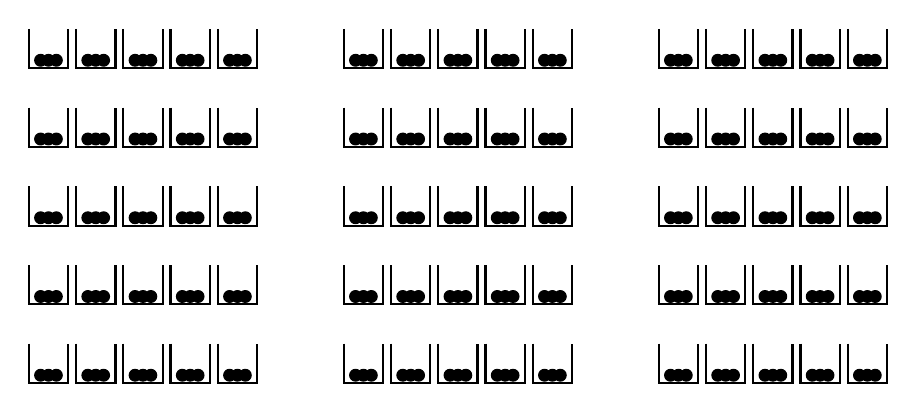
\begin{tikzpicture}[scale=0.5]
\newcommand\lax[3]{
\path[draw,thick,-] (#1-0.5,#2+0.5) -- (#1-0.5,#2-0.5) --
                    (#1+0.5,#2-0.5) -- (#1+0.5,#2+0.5);
\ifthenelse{\equal{#3}{1}}{\draw[fill=black] (#1,#2-0.3) circle (0.15);}{}
\ifthenelse{\equal{#3}{2}}{\draw[fill=black] (#1-0.2,#2-0.3) circle (0.15);}{}
\ifthenelse{\equal{#3}{2}}{\draw[fill=black] (#1+0.2,#2-0.3) circle (0.15);}{}
}
\newcommand\laa[7]{
    \lax{#1}{#2}{#3}
    \lax{#1+1.2}{#2}{#4}
    \lax{#1+2.4}{#2}{#5}
    \lax{#1+3.6}{#2}{#6}
    \lax{#1+4.8}{#2}{#7}
}

\laa{0}{0}{2}{0}{0}{0}{0}
\laa{0}{-2}{1}{1}{0}{0}{0}
\laa{0}{-4}{1}{0}{1}{0}{0}
\laa{0}{-6}{1}{0}{0}{1}{0}
\laa{0}{-8}{1}{0}{0}{0}{1}
\laa{8}{0}{0}{2}{0}{0}{0}
\laa{8}{-2}{0}{1}{1}{0}{0}
\laa{8}{-4}{0}{1}{0}{1}{0}
\laa{8}{-6}{0}{1}{0}{0}{1}
\laa{8}{-8}{0}{0}{2}{0}{0}
\laa{16}{0}{0}{0}{1}{1}{0}
\laa{16}{-2}{0}{0}{1}{0}{1}
\laa{16}{-4}{0}{0}{0}{2}{0}
\laa{16}{-6}{0}{0}{0}{1}{1}
\laa{16}{-8}{0}{0}{0}{0}{2}

\end{tikzpicture}
\end{center}

Prosessin voi kuvata merkkijonona, joka muodostuu
merkeistä ''o'' ja ''$\rightarrow$''.
Pallojen sijoittaminen alkaa
vasemmanpuoleisimmasta laatikosta.
Merkki ''o'' tarkoittaa, että pallo sijoitetaan
nykyiseen laatikkoon, ja merkki
''$\rightarrow$'' tarkoittaa, että siirrytään
seuraavaan laatikkoon.

Nyt jokainen sijoitustapa on merkkijono, jossa
on $k$ kertaa merkki ''o'' ja $n-1$ kertaa
merkki ''$\rightarrow$''.
Esimerkiksi sijoitustapaa
ylhäällä oikealla
vastaa merkkijono ''$\rightarrow$ $\rightarrow$ o $\rightarrow$ o $\rightarrow$''.
Niinpä sijoitustapojen määrä on ${k+n-1 \choose k}$.

\textit{Tapaus 3}: Kuhunkin laatikkoon saa sijoittaa
enintään yhden pallon ja lisäksi missään kahdessa
vierekkäisessä laatikossa ei saa olla palloa.
Esimerkiksi kun $n=5$ ja $k=2$, sijoitustapoja on 6:


\begin{center}
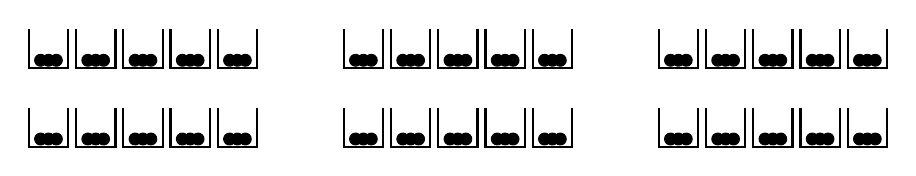
\begin{tikzpicture}[scale=0.5]
\newcommand\lax[3]{
\path[draw,thick,-] (#1-0.5,#2+0.5) -- (#1-0.5,#2-0.5) --
                    (#1+0.5,#2-0.5) -- (#1+0.5,#2+0.5);
\ifthenelse{\equal{#3}{1}}{\draw[fill=black] (#1,#2-0.3) circle (0.15);}{}
\ifthenelse{\equal{#3}{2}}{\draw[fill=black] (#1-0.2,#2-0.3) circle (0.15);}{}
\ifthenelse{\equal{#3}{2}}{\draw[fill=black] (#1+0.2,#2-0.3) circle (0.15);}{}
}
\newcommand\laa[7]{
    \lax{#1}{#2}{#3}
    \lax{#1+1.2}{#2}{#4}
    \lax{#1+2.4}{#2}{#5}
    \lax{#1+3.6}{#2}{#6}
    \lax{#1+4.8}{#2}{#7}
}

\laa{0}{0}{1}{0}{1}{0}{0}
\laa{0}{-2}{1}{0}{0}{1}{0}
\laa{8}{0}{1}{0}{0}{0}{1}
\laa{8}{-2}{0}{1}{0}{1}{0}
\laa{16}{0}{0}{1}{0}{0}{1}
\laa{16}{-2}{0}{0}{1}{0}{1}
\end{tikzpicture}
\end{center}

Tässä tapauksessa voi ajatella, että alussa $k$ palloa
ovat laatikoissaan ja joka välissä on yksi tyhjä laatikko.
Tämän jälkeen jää valittavaksi $n-k-(k-1)=n-2k+1$ tyhjän laatikon paikat.
Mahdollisia välejä on $k+1$, joten tapauksen 2 perusteella
sijoitustapoja on ${n-2k+1+k+1-1 \choose n-2k+1} = {n-k+1 \choose n-2k+1}$.

\subsubsection{Multinomikerroin}

\index{multinomikerroin@multinomikerroin}

Binomikertoimen yleistys on \key{multinomikerroin}

\[ {n \choose k_1,k_2,\ldots,k_m} = \frac{n!}{k_1! k_2! \cdots k_m!}, \]

missä $k_1+k_2+\cdots+k_m=n$.
Multinomikerroin ilmaisee, monellako tavalla $n$ alkiota voidaan jakaa osajoukkoihin,
joiden koot ovat $k_1,k_2,\ldots,k_m$.
Jos $m=2$, multinomikertoimen kaava vastaa binomikertoimen kaavaa.

\section{Catalanin luvut}

\index{Catalanin luku@Catalanin luku}

\key{Catalanin luku} $C_n$ ilmaisee,
montako tapaa on muodostaa kelvollinen sulkulauseke
$n$ alkusulusta ja $n$ loppusulusta.

Esimerkiksi $C_3=5$, koska 3 alkusulusta
ja 3 loppusulusta on mahdollista muodostaa
seuraavat kelvolliset sulkulausekkeet:

\begin{itemize}[noitemsep]
\item \texttt{()()()}
\item \texttt{(())()}
\item \texttt{()(())}
\item \texttt{((()))}
\item \texttt{(()())}
\end{itemize}

\subsubsection{Sulkulausekkeet}

\index{sulkulauseke@sulkulauseke}

Mikä sitten tarkkaan ottaen on
\textit{kelvollinen sulkulauseke}?
Seuraavat säännöt kuvailevat täsmällisesti
kaikki kelvolliset sulkulausekkeet:

\begin{itemize}
\item Sulkulauseke \texttt{()} on kelvollinen.
\item Jos sulkulauseke $A$ on kelvollinen,
niin myös sulkulauseke \texttt{(}$A$\texttt{)}
on kelvollinen.
\item Jos sulkulausekkeet $A$ ja $B$ ovat kelvollisia,
niin myös sulkulauseke $AB$ on kelvollinen.
\end{itemize}

Toinen tapa luonnehtia kelvollista sulkulauseketta on,
että jos valitaan mikä tahansa lausekkeen alkuosa,
niin alkusulkuja on ainakin yhtä monta
kuin loppusulkuja.
Lisäksi koko lausekkeessa
tulee olla tarkalleen yhtä monta
alkusulkua ja loppusulkua.

\subsubsection{Laskutapa 1}

Catalanin lukuja voi laskea rekursiivisesti kaavalla
\[ C_n = \sum_{i=0}^{n-1} C_{i} C_{n-i-1}.\]

Summa käy läpi tavat
jakaa sulkulauseke kahteen osaan niin,
että kumpikin osa on kelvollinen sulkulauseke
ja alkuosa on mahdollisimman lyhyt mutta ei tyhjä.
Kunkin vaihtoehdon kohdalla alkuosassa
on $i+1$ sulkuparia ja lausekkeiden määrä
saadaan kertomalla keskenään:

\begin{itemize}
\item $C_{i}$: tavat muodostaa sulkulauseke
alkuosan sulkupareista ulointa sulkuparia lukuun ottamatta
\item $C_{n-i-1}$: tavat muodostaa sulkulauseke
loppuosan sulkupareista
\end{itemize}
Lisäksi pohjatapauksena on $C_0=1$, koska 0
sulkuparista voi muodostaa
tyhjän sulkulausekkeen.

\subsubsection{Laskutapa 2}

Catalanin lukuja voi laskea myös binomikertoimen avulla:
\[ C_n = \frac{1}{n+1} {2n \choose n}\]
Kaavan voi perustella seuraavasti:

Kun käytössä on $n$ alkusulkua ja $n$ loppusulkua,
niistä voi muodostaa kaikkiaan ${2n \choose n}$
sulkulauseketta.
Lasketaan seuraavaksi, moniko tällainen
sulkulauseke \textit{ei} ole kelvollinen.

Jos sulkulauseke ei ole kelvollinen,
siinä on oltava alkuosa,
jossa loppusulkuja on alkusulkuja enemmän.
Muutetaan jokainen tällaisen alkuosan
sulkumerkki käänteiseksi.
Esimerkiksi lausekkeessa \texttt{())()(}
alkuosa on \texttt{())} ja kääntämisen
jälkeen lausekkeesta tulee \texttt{)((()(}.

Tuloksena olevassa lausekkeessa on $n+1$ alkusulkua
ja $n-1$ loppusulkua. Tällaisia lausekkeita on
kaikkiaan ${2n \choose n+1}$,
joka on sama kuin ei-kelvollisten
sulkulausekkeiden määrä.
Niinpä kelvollisten
sulkulausekkeiden määrä voidaan laskea kaavalla
\[{2n \choose n}-{2n \choose n+1} = {2n \choose n} - \frac{n}{n+1} {2n \choose n} = \frac{1}{n+1} {2n \choose n}.\]

\subsubsection{Puiden laskeminen}

Catalanin luvut kertovat myös juurellisten
puiden lukumääriä:

\begin{itemize}
\item $n$ solmun binääripuiden määrä on $C_n$
\item $n$ solmun juurellisten puiden määrä on $C_{n-1}$
\end{itemize}
\noindent
Esimerkiksi tapauksessa $C_3=5$ binääripuut ovat

\begin{center}
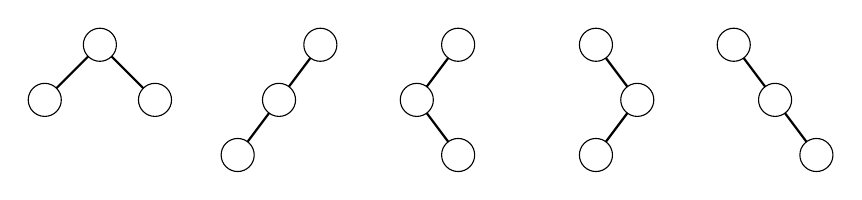
\begin{tikzpicture}[scale=0.7]
\path[draw,thick,-] (0,0) -- (-1,-1);
\path[draw,thick,-] (0,0) -- (1,-1);
\draw[fill=white] (0,0) circle (0.3);
\draw[fill=white] (-1,-1) circle (0.3);
\draw[fill=white] (1,-1) circle (0.3);

\path[draw,thick,-] (4,0) -- (4-0.75,-1) -- (4-1.5,-2);
\draw[fill=white] (4,0) circle (0.3);
\draw[fill=white] (4-0.75,-1) circle (0.3);
\draw[fill=white] (4-1.5,-2) circle (0.3);

\path[draw,thick,-] (6.5,0) -- (6.5-0.75,-1) -- (6.5-0,-2);
\draw[fill=white] (6.5,0) circle (0.3);
\draw[fill=white] (6.5-0.75,-1) circle (0.3);
\draw[fill=white] (6.5-0,-2) circle (0.3);

\path[draw,thick,-] (9,0) -- (9+0.75,-1) -- (9-0,-2);
\draw[fill=white] (9,0) circle (0.3);
\draw[fill=white] (9+0.75,-1) circle (0.3);
\draw[fill=white] (9-0,-2) circle (0.3);

\path[draw,thick,-] (11.5,0) -- (11.5+0.75,-1) -- (11.5+1.5,-2);
\draw[fill=white] (11.5,0) circle (0.3);
\draw[fill=white] (11.5+0.75,-1) circle (0.3);
\draw[fill=white] (11.5+1.5,-2) circle (0.3);
\end{tikzpicture}
\end{center}
ja juurelliset puut ovat
\begin{center}
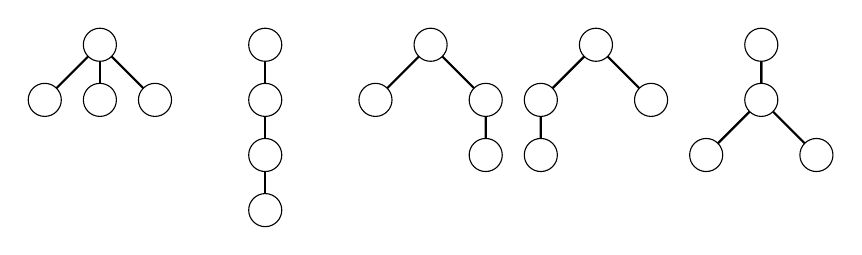
\begin{tikzpicture}[scale=0.7]
\path[draw,thick,-] (0,0) -- (-1,-1);
\path[draw,thick,-] (0,0) -- (0,-1);
\path[draw,thick,-] (0,0) -- (1,-1);
\draw[fill=white] (0,0) circle (0.3);
\draw[fill=white] (-1,-1) circle (0.3);
\draw[fill=white] (0,-1) circle (0.3);
\draw[fill=white] (1,-1) circle (0.3);

\path[draw,thick,-] (3,0) -- (3,-1) -- (3,-2) -- (3,-3);
\draw[fill=white] (3,0) circle (0.3);
\draw[fill=white] (3,-1) circle (0.3);
\draw[fill=white] (3,-2) circle (0.3);
\draw[fill=white] (3,-3) circle (0.3);

\path[draw,thick,-] (6+0,0) -- (6-1,-1);
\path[draw,thick,-] (6+0,0) -- (6+1,-1) -- (6+1,-2);
\draw[fill=white] (6+0,0) circle (0.3);
\draw[fill=white] (6-1,-1) circle (0.3);
\draw[fill=white] (6+1,-1) circle (0.3);
\draw[fill=white] (6+1,-2) circle (0.3);

\path[draw,thick,-] (9+0,0) -- (9+1,-1);
\path[draw,thick,-] (9+0,0) -- (9-1,-1) -- (9-1,-2);
\draw[fill=white] (9+0,0) circle (0.3);
\draw[fill=white] (9+1,-1) circle (0.3);
\draw[fill=white] (9-1,-1) circle (0.3);
\draw[fill=white] (9-1,-2) circle (0.3);

\path[draw,thick,-] (12+0,0) -- (12+0,-1) -- (12-1,-2);
\path[draw,thick,-] (12+0,0) -- (12+0,-1) -- (12+1,-2);
\draw[fill=white] (12+0,0) circle (0.3);
\draw[fill=white] (12+0,-1) circle (0.3);
\draw[fill=white] (12-1,-2) circle (0.3);
\draw[fill=white] (12+1,-2) circle (0.3);

\end{tikzpicture}
\end{center}


\section{Inkluusio-ekskluusio}

\index{inkluusio-ekskluusio}

\key{Inkluusio-ekskluusio}
on tekniikka, jonka avulla pystyy laskemaan
joukkojen yhdisteen koon leikkausten
kokojen perusteella ja päinvastoin.
Yksinkertainen esimerkki periaatteesta on kaava
\[ |A \cup B| = |A| + |B| - |A \cap B|,\]
jossa $A$ ja $B$ ovat joukkoja ja $|X|$
tarkoittaa joukon $X$ kokoa.
Seuraava kuva havainnollistaa kaavaa,
kun joukot ovat tason ympyröitä:

\begin{center}
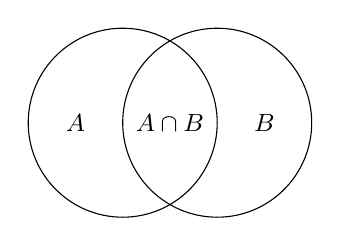
\begin{tikzpicture}[scale=0.8]

\draw (0,0) circle (1.5);
\draw (1.5,0) circle (1.5);

\node at (-0.75,0) {\small $A$};
\node at (2.25,0) {\small $B$};
\node at (0.75,0) {\small $A \cap B$};

\end{tikzpicture}
\end{center}

Tavoitteena on laskea, kuinka suuri on yhdiste $A \cup B$
eli alue, joka on toisen tai kummankin ympyrän sisällä.
Kuvan mukaisesti yhdisteen $A \cup B$ koko
saadaan laskemalla ensin yhteen ympyröiden $A$ ja $B$ koot
ja vähentämällä siitä sitten leikkauksen $A \cap B$ koko.

Samaa ideaa voi soveltaa, kun joukkoja on enemmän.
Kolmen joukon tapauksessa kaavasta tulee
\[ |A \cup B \cup C| = |A| + |B| + |C| - |A \cap B|  - |A \cap C|  - |B \cap C| + |A \cap B \cap C| \]
ja vastaava kuva on

\begin{center}
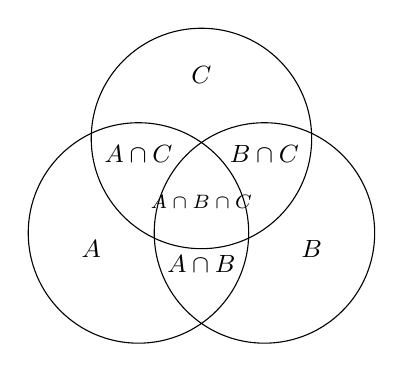
\begin{tikzpicture}[scale=0.8]

\draw (0,0) circle (1.75);
\draw (2,0) circle (1.75);
\draw (1,1.5) circle (1.75);

\node at (-0.75,-0.25) {\small $A$};
\node at (2.75,-0.25) {\small $B$};
\node at (1,2.5) {\small $C$};
\node at (1,-0.5) {\small $A \cap B$};
\node at (0,1.25) {\small $A \cap C$};
\node at (2,1.25) {\small $B \cap C$};
\node at (1,0.5) {\scriptsize $A \cap B \cap C$};

\end{tikzpicture}
\end{center}

Yleisessä tapauksessa yhdisteen $X_1 \cup X_2 \cup \cdots \cup X_n$
koon saa laskettua käymällä läpi kaikki tavat muodostaa
leikkaus joukoista $X_1,X_2,\ldots,X_n$.
Parittoman määrän joukkoja sisältävät leikkaukset
lasketaan mukaan positiivisina ja
parillisen määrän negatiivisina.

Huomaa, että vastaavat kaavat toimivat myös käänteisesti
leikkauksen koon laskemiseen yhdisteiden kokojen perusteella.
Esimerkiksi
\[ |A \cap B| = |A| + |B| - |A \cup B|\]
ja
\[ |A \cap B \cap C| = |A| + |B| + |C| - |A \cup B|  - |A \cup C|  - |B \cup C| + |A \cup B \cup C| .\]

\subsubsection{Epäjärjestykset}

\index{epxjxrjestys@epäjärjestys}

Lasketaan esimerkkinä,
montako tapaa on muodostaa luvuista
$(1,2,\ldots,n)$ \key{epäjärjestys}
eli permutaatio,
jossa mikään luku ei ole alkuperäisellä paikallaan.
Esimerkiksi jos $n=3$, niin epäjärjestyksiä on kaksi: $(2,3,1)$ ja $(3,1,2)$.

Yksi tapa lähestyä tehtävää on käyttää inkluusio-ekskluusiota.
Olkoon joukko $X_k$ niiden permutaatioiden joukko,
jossa kohdassa $k$ on luku $k$.
Esimerkiksi jos $n=3$, niin joukot ovat seuraavat:
\[
\begin{array}{lcl}
X_1 & = & \{(1,2,3),(1,3,2)\} \\
X_2 & = & \{(1,2,3),(3,2,1)\} \\
X_3 & = & \{(1,2,3),(2,1,3)\} \\
\end{array}
\]
Näitä joukkoja käyttäen epäjärjestysten määrä on
\[ n! - |X_1 \cup X_2 \cup \cdots \cup X_n|, \]
eli
riittää laskea joukkojen yhdisteen koko.
Tämä palautuu inkluusio-eks\-kluu\-sion avulla
joukkojen leikkausten kokojen laskemiseen,
mikä onnistuu tehokkaasti.
Esimerkiksi kun $n=3$, joukon $|X_1 \cup X_2 \cup X_3|$ koko on
\[
\begin{array}{lcl}
 & & |X_1| + |X_2| + |X_3| - |X_1 \cap X_2|  - |X_1 \cap X_3|  - |X_2 \cap X_3| + |X_1 \cap X_2 \cap X_3| \\
 & = & 2+2+2-1-1-1+1 \\
 & = & 4, \\
\end{array}
\]
joten ratkaisujen määrä on $3!-4=2$.

Osoittautuu, että tehtävän voi ratkaista myös toisella
tavalla käyttämättä inkluusio-ekskluusiota.
Merkitään $f(n)$:llä jonon $(1,2,\ldots,n)$ epäjärjestysten määrää,
jolloin seuraava rekursio pätee:

\begin{equation*}
    f(n) = \begin{cases}
               0               & n = 1\\
               1               & n = 2\\
               (n-1)(f(n-2) + f(n-1)) & n>2 \\
           \end{cases}
\end{equation*}

Kaavan voi perustella käymällä läpi tapaukset,
miten luku 1 muuttuu epäjärjestyksessä.
On $n-1$ tapaa valita jokin luku $x$ luvun 1 tilalle.
Jokaisessa tällaisessa valinnassa on kaksi vaihtoehtoa:

\textit{Vaihtoehto 1:} Luvun $x$ tilalle valitaan luku 1.
Tällöin jää $n-2$ lukua, joille tulee muodostaa epäjärjestys.

\textit{Vaihtoehto 2:} Luvun $x$ tilalle ei valita lukua 1.
Tällöin jää $n-1$ lukua, joille tulee muodostaa epäjärjestys,
koska luvun $x$ tilalle ei saa valita lukua 1
ja kaikki muut luvut tulee saattaa epäjärjestykseen.

\section{Burnsiden lemma}

\index{Burnsiden lemma@Burnsiden lemma}

\key{Burnsiden lemma} laskee yhdistelmien määrän niin,
että symmetrisistä yhdistelmistä lasketaan
mukaan vain yksi edustaja.
Burnsiden lemman mukaan yhdistelmien määrä on
\[\sum_{k=1}^n \frac{c(k)}{n},\]
missä yhdistelmän asentoa voi muuttaa $n$ tavalla
ja $c(k)$ on niiden yhdistelmien määrä,
jotka pysyvät ennallaan, kun asentoa
muutetaan tavalla $k$.

Lasketaan esimerkkinä, montako
erilaista tapaa on
muodostaa $n$ helmen helminauha,
kun kunkin helmen värin tulee olla
väliltä $1,2,\ldots,m$.
Kaksi helminauhaa ovat symmetriset,
jos ne voi saada näyttämään samalta pyörittämällä.
Esimerkiksi helminauhan
\begin{center}
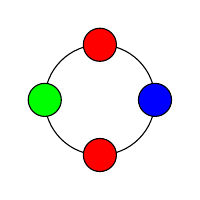
\begin{tikzpicture}[scale=0.7]
\draw[fill=white] (0,0) circle (1);
\draw[fill=red] (0,1) circle (0.3);
\draw[fill=blue] (1,0) circle (0.3);
\draw[fill=red] (0,-1) circle (0.3);
\draw[fill=green] (-1,0) circle (0.3);
\end{tikzpicture}
\end{center}
kanssa symmetriset helminauhat ovat seuraavat:
\begin{center}
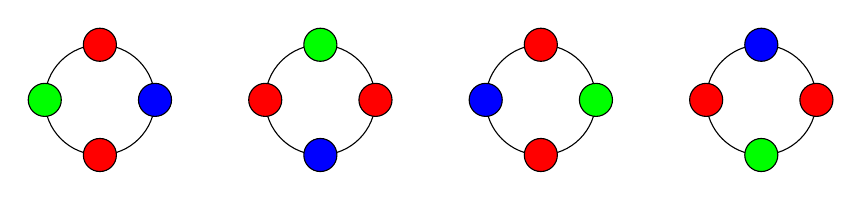
\begin{tikzpicture}[scale=0.7]
\draw[fill=white] (0,0) circle (1);
\draw[fill=red] (0,1) circle (0.3);
\draw[fill=blue] (1,0) circle (0.3);
\draw[fill=red] (0,-1) circle (0.3);
\draw[fill=green] (-1,0) circle (0.3);

\draw[fill=white] (4,0) circle (1);
\draw[fill=green] (4+0,1) circle (0.3);
\draw[fill=red] (4+1,0) circle (0.3);
\draw[fill=blue] (4+0,-1) circle (0.3);
\draw[fill=red] (4+-1,0) circle (0.3);

\draw[fill=white] (8,0) circle (1);
\draw[fill=red] (8+0,1) circle (0.3);
\draw[fill=green] (8+1,0) circle (0.3);
\draw[fill=red] (8+0,-1) circle (0.3);
\draw[fill=blue] (8+-1,0) circle (0.3);

\draw[fill=white] (12,0) circle (1);
\draw[fill=blue] (12+0,1) circle (0.3);
\draw[fill=red] (12+1,0) circle (0.3);
\draw[fill=green] (12+0,-1) circle (0.3);
\draw[fill=red] (12+-1,0) circle (0.3);
\end{tikzpicture}
\end{center}
Tapoja muuttaa asentoa on $n$,
koska helminauhaa voi pyörittää $0,1,\ldots,n-1$
askelta myötäpäivään.
Jos helminauhaa pyörittää 0 askelta,
kaikki $m^n$ väritystä säilyvät ennallaan.
Jos taas helminauhaa pyörittää 1 askeleen,
vain $m$ yksiväristä helminauhaa säilyy ennallaan.

Yleisemmin kun helminauhaa pyörittää $k$ askelta,
ennallaan säilyvien yhdistelmien määrä on
\[m^{\textrm{syt}(k,n)},\]
missä $\textrm{syt}(k,n)$ on lukujen $k$ ja $n$
suurin yhteinen tekijä.
Tämä johtuu siitä, että $\textrm{syt}(k,n)$-kokoiset
pätkät helmiä siirtyvät toistensa paikoille
$k$ askelta eteenpäin.
Niinpä helminauhojen määrä on
Burnsiden lemman mukaan
\[\sum_{i=0}^{n-1} \frac{m^{\textrm{syt}(i,n)}}{n}. \]
Esimerkiksi kun helminauhan pituus on 4
ja värejä on 3, helminauhoja on
\[\frac{3^4+3+3^2+3}{4} = 24. \]

\section{Cayleyn kaava}

\index{Cayleyn kaava@Cayleyn kaava}

\key{Cayleyn kaavan} mukaan $n$ solmusta voi
muodostaa $n^{n-2}$ numeroitua puuta.
Puun solmut on numeroitu $1,2,\ldots,n$,
ja kaksi puuta ovat erilaiset,
jos niiden rakenne on erilainen
tai niissä on eri numerointi.

\begin{samepage}
\noindent
Esimerkiksi kun $n=4$, numeroitujen puiden määrä on $4^{4-2}=16$:

\begin{center}
\begin{tikzpicture}[scale=0.8]
\footnotesize

\newcommand\puua[6]{
\path[draw,thick,-] (#1,#2) -- (#1-1.25,#2-1.5);
\path[draw,thick,-] (#1,#2) -- (#1,#2-1.5);
\path[draw,thick,-] (#1,#2) -- (#1+1.25,#2-1.5);
\node[draw, circle, fill=white] at (#1,#2) {#3};
\node[draw, circle, fill=white] at (#1-1.25,#2-1.5) {#4};
\node[draw, circle, fill=white] at (#1,#2-1.5) {#5};
\node[draw, circle, fill=white] at (#1+1.25,#2-1.5) {#6};
}
\newcommand\puub[6]{
\path[draw,thick,-] (#1,#2) -- (#1+1,#2);
\path[draw,thick,-] (#1+1,#2) -- (#1+2,#2);
\path[draw,thick,-] (#1+2,#2) -- (#1+3,#2);
\node[draw, circle, fill=white] at (#1,#2) {#3};
\node[draw, circle, fill=white] at (#1+1,#2) {#4};
\node[draw, circle, fill=white] at (#1+2,#2) {#5};
\node[draw, circle, fill=white] at (#1+3,#2) {#6};
}

\puua{0}{0}{1}{2}{3}{4}
\puua{4}{0}{2}{1}{3}{4}
\puua{8}{0}{3}{1}{2}{4}
\puua{12}{0}{4}{1}{2}{3}

\puub{0}{-3}{1}{2}{3}{4}
\puub{4.5}{-3}{1}{2}{4}{3}
\puub{9}{-3}{1}{3}{2}{4}
\puub{0}{-4.5}{1}{3}{4}{2}
\puub{4.5}{-4.5}{1}{4}{2}{3}
\puub{9}{-4.5}{1}{4}{3}{2}
\puub{0}{-6}{2}{1}{3}{4}
\puub{4.5}{-6}{2}{1}{4}{3}
\puub{9}{-6}{2}{3}{1}{4}
\puub{0}{-7.5}{2}{4}{1}{3}
\puub{4.5}{-7.5}{3}{1}{2}{4}
\puub{9}{-7.5}{3}{2}{1}{4}
\end{tikzpicture}
\end{center}
\end{samepage}

Seuraavaksi näemme, miten Cayleyn kaavan
voi perustella samastamalla numeroidut puut
Prüfer-koodeihin.

\subsubsection{Prüfer-koodi}

\index{Prüfer-koodi}

\key{Prüfer-koodi} on $n-2$ luvun jono,
joka kuvaa numeroidun puun rakenteen.
Koodi muodostuu poistamalla puusta
joka askeleella lehden, jonka numero on pienin,
ja lisäämällä lehden vieressä olevan solmun
numeron koodiin.

Esimerkiksi puun
\begin{center}
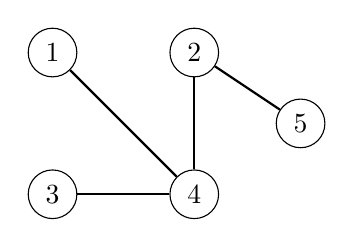
\begin{tikzpicture}[scale=0.9]
\node[draw, circle] (1) at (2,3) {$1$};
\node[draw, circle] (2) at (4,3) {$2$};
\node[draw, circle] (3) at (2,1) {$3$};
\node[draw, circle] (4) at (4,1) {$4$};
\node[draw, circle] (5) at (5.5,2) {$5$};

%\path[draw,thick,-] (1) -- (2);
%\path[draw,thick,-] (1) -- (3);
\path[draw,thick,-] (1) -- (4);
\path[draw,thick,-] (3) -- (4);
\path[draw,thick,-] (2) -- (4);
\path[draw,thick,-] (2) -- (5);
%\path[draw,thick,-] (4) -- (5);
\end{tikzpicture}
\end{center}
Prüfer-koodi on $[4,4,2]$,
koska puusta poistetaan ensin solmu 1,
sitten solmu 3 ja lopuksi solmu 5.

Jokaiselle puulle voidaan laskea
Prüfer-koodi, minkä lisäksi
Prüfer-koodista pystyy palauttamaan
yksikäsitteisesti alkuperäisen puun.
Niinpä numeroituja puita on yhtä monta
kuin Prüfer-koodeja eli $n^{n-2}$.

